\documentclass[conference]{IEEEtran}
\IEEEoverridecommandlockouts
% The preceding line is only needed to identify funding in the first footnote. If that is unneeded, please comment it out.
\usepackage{cite}
\usepackage{amsmath,amssymb,amsfonts}
\usepackage{algorithmicx}
\usepackage{graphicx, algorithm, algpseudocode}
\usepackage{textcomp}
\usepackage{xcolor}
\usepackage{url}
\def\BibTeX{{\rm B\kern-.05em{\sc i\kern-.025em b}\kern-.08em
    T\kern-.1667em\lower.7ex\hbox{E}\kern-.125emX}}
\begin{document}

\title{The Decision Making of Autonomous Vehicles: A Survey}

\author{\IEEEauthorblockN{Wenxing Lan}
\IEEEauthorblockA{\textit{Department of Computer Science and Engineering} \\
\textit{Southern University of Science and Technology}\\
Shenzhen, China. \\
12032882@mail.sustech.edu.cn}


}

\maketitle

\begin{abstract}

\end{abstract}

\begin{IEEEkeywords}
component, formatting, style, styling, insert
\end{IEEEkeywords}

\section{Introduction}
Autonomous vehicles (also known as self-driving vehicles and driverless vehicles) have been researched by many universities, research institutes, internet companies, vehicle companies and companies of other industries around the world since the middle 1980s~\cite{self_driving}. In the last two decades, several crucial of autonomous vehicle research platforms are as follows: the Navlab's mobile platform~\cite{Thorpe199144}, University of Pavia's and Parma's car, ARGO~\cite{Broggi199955}, and UBM's vehicles, VaMoRs and VaMP~\cite{Gregor200248}.

In the last decade, the Defence Advanced Research Projects Agency (DARPA) organized three competitions to accelerate the development of correlation technique about autonomous vehicles~\cite{Brian2016}. In 2004, the first competition named as DARPA Grand Challenge was held in the Mojave Desert, USA~\cite{self_driving}. The goal is to get autonomous vehicles to travel 140 miles of off-road routes as fast as possible~\cite{Brian2016}. Unfortunately, there is no autonomous vehicle which was able to complete the whole journey~\cite{self_driving}.

In 2005, the DARPA Grand Challenge was held again and required autonomous vehicles to travel 132 miles of difficult desert roads across Nevada which contain a mixture of featureless terrain, dust, global positioning system drop-outs, sharp turns, narrow openings, bridges, railroad overpasses, long tunnels, obstacles and a narrow winding mountains road with a 200-foot drop-off~\cite{Buehler2007}. This competition had 23 finalists and 4 cars finished the course within 10-hour limit. Remarkably, the Stanford University's vehicles, Stanley, won the first-place prize, and the Carnegie Mellon University's cars, Sandstorm and H1ghlander, came in second and third place, respectively~\cite{Buehler2007}.

The third competition which is named as the DARPA Urban Challenge was held at the now-closed George Air Force Base, California, USA, in 2007. The objective was for a autonomous vehicles to complete the 60 mile course in less than 6 hours. Additionally, the autonomous vehicles were asked to obey all traffic regulations which avoiding other vehicles including driverless and humandriven vehicles~\cite{buehler2009darpa}. There are 11 finalists in this competition and 6 vehicles completed the route within the allotted time limit. Specifically, Boss, the vehicle of Carnegie Mellon University, won the first-place prize, the Stanford University's car, Junior, claimed second place, and the Virginia Tech's car, Odin, finished in third~\cite{buehler2009darpa}. Although the challenges presented by these competitions cannot cover all the challenges encountered in everyday traffic, they have been hailed as milestones in the development of autonomous vehicles~\cite{Brian2016}.

After the DARPA Challenge, there was a flood of driverless events. Relevant examples include: Intelligent Vehicle Future Challenges~\cite{xin2014china}, from 2009 to 2013; Hyundai Autonomous Challenge~\cite{Cerri2011}, which was held in 2010; VisLab Intercontinental Autonomous Challenge~\cite{broggi2012vislab}, in 2010; the Grand Cooperative Driving Challenge (GCDC)~\cite{Englund2016}, in 2011 and 2016 and Public Road Urban Driverless-Car Test~\cite{Broggi2015}, which was held in 2013. At the same time, many industrial and academic teams have invested a lot of research and development energy in the field of autonomous driving. Among them, the industry is represented by the OEMs of Ford, Toyota, Hyundai and other car companies, as well as IT and emerging companies such as Waymo, Tesla, Uber, Intel, Baidu, Pony.ai, etc., and have developed various autonomous vehicle platforms based on commercialization goals; Academia, including CMU, Stanford, UC Berkeley, Tsinghua University, Tongji University, Southern University of Science and Technology and other major domestic and foreign universities have carried out a series of researches around the key technical fields of autonomous driving.

In order to regulate the application of unmanned driving technology, the National Highway Transportation Safety Administration of the United States Department of Transportation has divided the level of automatic driving (based on the SAE International Standard J3016~\cite{sae2018taxonomy}):
\begin{enumerate}
	\item Level 0 (manual driving): completely controlled by a human driver;
	\item Level 1 (assisted driving): The driving environment provides support for one of the steering wheel and acceleration and deceleration operations, and the rest is operated by humans. Contains basic auxiliary driving, such as adaptive cruise control (ACC), anti-lock brake system (ABS), electronic stability control system (ESC);
	\item Level 2 (semi-automatic driving): The driving environment provides support for multiple operations in the steering wheel and acceleration and deceleration, and the rest is operated by humans.  Contains some advanced auxiliary driving functions, such as a horizontal/vertical control system with minimal risk, emergency braking, etc.;
	\item Level 3 (Highly Autonomous Driving): The unmanned driving system completes all operations, but requires the human driver to take over when leaving the operational scene of unmanned driving.
	\item Level 4 (Ultra-high auto-driving): An unmanned driving system with limited roads and environmental conditions, and does not require human drivers to respond to system requests.
	\item Level 5 (Fully Automated Driving): Unmanned driving system that does not limit roads and environmental conditions
\end{enumerate}

The perception system and the decision-making system are two main parts of the autonomy system architecture of autonomous vehicle~\cite{Brian2016}. To limit the scope of this survey, We focus on some aspects of decision-making system, which includes route planning, path planning, behavior selection, motion planning, obstacle avoidance and control, in particular, for systems falling into the automation level of 3 and above~\cite{self_driving}.
The remainder of the paper id structured as follows:
\begin{enumerate}
	\item Overview of the Decision-Making Hierarchy
	\item Route planning
	\item Path planning
	\item Behavior selector
	\item Motion planning
	\item Obstacle Avoidance and control
	\item Conclusion
\end{enumerate}


\section{Overview of the Decision-Making Hierarchy}

\begin{figure}[htbp]
	\centering
	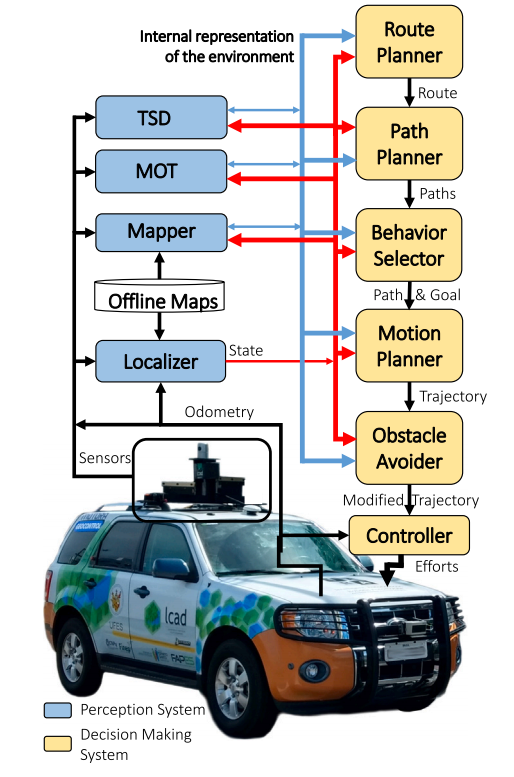
\includegraphics[width=1\columnwidth]{./picture/architecture.png}
	\caption{\label{architecture}
		The five subsystems of decision making system of a typical autonomous vehicle.}
\end{figure}

In this section, the decision making system of a typical autonomous vehicles is described and the brief description of each component of decision making system is provided. The perception system of autonomous vehicles use data captured by on-board sensors, such as Light Detection and Ranging (LIDAR), Radio Detection and Ranging (RADAR), camera, Global Positioning System (GPS), Inertial Measurement Unit (IMU), odometer, etc., and prior information about the models of sensors, road network, traffic rules, vehicle dynamics, etc. to estimate the state of vehicles and create representation of the surrounding environment~\cite{self_driving}. Then, the decision making system use the estimation and environment constructed to control the vehicle in order to reach the goal object~\cite{Brian2016}. 

There are six subsystems which are shown as the orange blocks in Fig~\ref{architecture} in the decision making system of a typical autonomous vehicles~\cite{self_driving}. The brief description of each subsystem is shown as belows.

\subsection{Route Planning Subsystem}
Given a requested destination defined in the road network by the user, the route planning subsystem aims to compute a route, $R$, through the road network from its current position to the requested destination~\cite{Brian2016}. A route, $R=\{r_1, r_2,...,r_{|R|}\}$, is a sequence of way point, where each way point, $r_i$ where $i \in \{1,2,...,|R|\}$, is a coordinate pair. i.e. $r_i = (x_i, y_i)$, in the road network~\cite{self_driving}. Actually, route palnning is a kind of global route planning since it needs to find the complete route from ego vehicle's current position to the final goal, such as the route planned by the BAIDU maps\footnote{https://map.baidu.com/}. The related methods for route planning is shown is Section~\ref{sec:route_planner}.

\subsection{Path Planning Subsystem}
Given a route computed by the route planning subsystem, the path planning subsystem computes a set of paths, $P=\{P_1, P_2, ..., P_{|P|}\}$ by considering the ego vehicle's current state and the traffic rules as well as the surrounding environment~\cite{self_driving}. A path is a sequence of poses, i.e. $P_j=\{p_1, p_2, ..., p_{|P_j|}\}$ where $j \in \{1, 2,...,|P|\}$~\cite{self_driving}. Additionally, each pose, $p_i$, is a coordinate tuple in the static map which only has static object, such as static obstacles, buildings and roads, aroung the ego vehicle and the desired vehicle's orientation at the position defined by this tuple, i.e., $p_i=(x_i, y_i, \theta_i)$~\cite{self_driving}. The relevant methods used in path planning subsystem will be given in Section~\ref{sec:path_planner}.

\subsection{Behavior Selection Subsystem}
The behavior selection subsystem is responsible to select the current reasonable driving behavior for the vehicle according to the behavior, traffic rules and road conditions of the current surrounding traffic participants~\cite{Brian2016}. The behaviors output here are specific driving maneuvers, such as acceleration and deceleration, lane change, overtaking, and following~\cite{Brian2016}. Additionally, the behavior selection subsystem need to select a pose in a selecting path among a set of paths generated by path palnning subsystem a few seconds ahead of the current ego vehicle's state~\cite{self_driving}. The relevant methods used in Path Behavior Selector is shown in Section~\ref{sec:behavior_selector}.

\subsection{Motion Planning Subsystem}
When the behavior is selected by the behavior selection subsystem (for example, it may be lane changing or left turning), motion planning subsystem needs to find a trajectory $T$ which is form the current ego vehicle's state to the curent goal state~\cite{Brian2016}. More importantly, the trajectory needs to satisfy the kinematic and dynamic constraints and be confortable for passengers~\cite{self_driving}. The trajectory $T=\{c_1, c_2, ..., c_{|T|}\}$ can be defined as a sequence of commands, $c_k=(v_k, \phi_k, \Delta_{t_k})$, where $v_k$ denotes the desired velocity at time $k$, $\phi_k$ represents the desired steering angle at time $k$, and $\Delta_{t_k}$ is the duration of $c_k$~\cite{self_driving}. In Section~\ref{sec:motion_planner}, the detail of methods used in motion planning subsystem will be given.

\subsection{Obstacle Avoidance Subsystem}
The obstacle avoidance subsytem needs to change the trajectory (usually decreasing the speed) which is the output of motion planning subsystem in order to avoid collision with other obstacle~\cite{self_driving}.  There is little literature on how to perform the function of this subsystem. Some of the literature related to this subsystem will be discussed in Section~\ref{sec:obstacle_avoider}.


\section{Related Work of Route Planning Subsystem}\label{sec:route_planner}
In this section, the related techniques reported in the literature for the Route Planning subsystem will be surveyed.

The road network, which is the input of the route planning subsystem, is usually represented as a weighted directed graph $G=(V, E)$~\cite{self_driving}. As a assumption, the weight of each edge is always a nonnegative value. In weighted directed graph $G$, each vertex $v_i$ where $v_i \in V=\{v_1, v_2, ..., v_{|V|}\}$ is road junction, such as crossroads, three forks, etc., and each directed edge $e_{ij}$ where $e_{i,j} \in E, i \neq j$ connects pairs of road junctions $v_i$ and $v_j$. Specifically, edge weight $w_{ij}$ denotes the cost of traversing edge $e_{ij}$. Computing a route, the task of route planning subsystem, can be reduced to find a path in a weighted directed graph. Normally, the path should be shorest since most users are willing to reach destination as soon as possible~\cite{self_driving}. Unfortunately, classical shortest path algorithms, such as Dijkstra~\cite{dijkstra1959note} and $A^*$~\cite{Hart1968formal} are impractical because of their high time complexity to large road networks, such as city road network or even nation road network~\cite{self_driving}.

The performance of route planning algorithms in road networks has improved significantly in the past decade~\cite{self_driving}. The driving direction can be calculated by some newly developed algorithm in milliseconds or less, even at national scale~\cite{bast2016route}. Various technologies supply different balance between preprocessing effort, query time and space usage~\cite{bast2016route}. The queries can be responded in less than a microsecond by some alforihtms, while the real-time traffic can be effectively handled by other algorithm~\cite{bast2016route}. The techniques used in route planning in a road network can be divided into six classes~\cite{bast2016route}:
\begin{enumerate}
	\item Basic Techniques
	\item Goal-directed Techniques
	\item Separator-based Techniques
	\item Hierachical Techniques
\end{enumerate}

\subsection{Basic Techniques}\label{subsec:basic_techniques}
Dijkstra's algorithm provides a standard solution to the one-to-all shortest path problem in a weighted directed graph, and pesudo code of Dijkstra's algorithm is shown in Algorithm~\ref{dijkstra}~\cite{dijkstra1959note}. \emph{label-setting}, one of the property of Dijkstra's algorithm, means that the traversing cost from start site $v_s$ to destination site $v_e$ is shortest once the destination site $v_e$ has been scanned~\cite{dijkstra1959note}. Consequently, the algorithm can be stopped as soon as it has been scanned the destination site for one-to-one queries~\cite{bast2016route}. The time complexity of Dijkstra's algorithm is influenced by the using priority queue. For example, the time complexity is $O((|V|+|E|)log|V|)$ if the priority queue is binary heaps~\cite{forsythe1964algorithms}.
\begin{algorithm}[htbp]
	\caption{\label{dijkstra}Dijkstra's Algorithm~\cite{dijkstra1959note}.}
	{\bf Input:} weighted directed graph $G=(V, E)$; start vertex $v_s \in V$
	\begin{algorithmic}[1]
		\State Initial a priority queue $Q=\{v_s\}$ of vertices which is ordered by total traversing cost from $v_s$.
		\State Initial all traversing cost $cost(v_s, v_i)=+\infty$ where $v_i \in V$.
		\State Set $cost(v_s, v_s) = 0$.
		\While {not all vertex $v \in V$ has been traversed}
			\State Exact a vertex $u$ with minimum traversing cost from $Q$.
			\State Find all arcs $E' = \{e | e=(u, v) \in E\}$ incident to $u$.
			\For {each $e=(u,v) \in E'$}
				\If {$cost(v_s, u)+w(u,v) < cost(v_s, v)$}
					\State Set $cost(v_s, v) = cost(v_s, u)+w(u,v)$.
				\EndIf
			\State Add $u$ into $Q$.
			\EndFor
			
		\EndWhile
		\State Return all traversing cost.
	\end{algorithmic}
\end{algorithm}

Bellman-Ford algorithm is an alternative method which can compute shortest path in a weighted directed graph~\cite{bellman1958routing, ford1956network}. At each iteration, it scans all vertices whose traversing cost have improve~\cite{bellman1958routing, ford1956network}. It often uses a simple FIFO queue to keep track of vertices to scan next~\cite{bast2016route}.  Additionally, Bellman-Ford algorithm has the \emph{label-correcting} property: each vertex may be scanned many times, and the time complexity of this algorithm is $O(|V||E|)$. Finally, the Floyd-Warshall algorithm calculates traversing cost between all pairs of vertices in $O(|V|^3)$ time~\cite{floyd1962algorithm}. It is more suitable for sufficiently dense graphs than Dijkstra's algorithm~\cite{bast2016route}.

In summary, these algorithm metioned above are the basic algorithm to find shortest path in a weighted directed graph. Although they all have high time complexity, they always can find one shortest path in a given nonegative weighted directed graph.
                         
\subsection{Goal-directed Techniques}
By avoiding scanning the vertices that are not in the direction of the target vertex, the goal-directed technology guides the search from the source vertex to the target vertex~\cite{bast2016route}.

$A^*$ algorithm, a classic goal-directed shortest path algorithm, uses a heuristic function $f(u,t)$ to estimate the traversing cost from vertex $u$ to $t$ ($t$ is usually the destination site.)~\cite{Hart1968formal}. Normally, the value of $f(u,t)$ is the lower bound of the traversing cost from vertex $u$ to $t$. Then, it runs a modified version of Dijkstra's algorithm which regards the value computed by the formula $cost(v_s, u)+f(u,t)$ as the prioirty of a vertex $u$~\cite{bast2016route}. Therefore, the vertices which are much closer to the destiniation site $t$ will be scanned earier during the implementation of the algorithm~\cite{bast2016route}. ALT ($A^*$, landmarks, and triangle inequality) algorithm uses inequality property among landmarks to automatically obtain a heuristic function with better lower bounds in order to replace the user-defined heuric function in $A^*$ algorithm~\cite{goldberg2005computing}. 

Arc flags, an another goal-directed method, needs to divide the grah into $C$ cells which are roughly balanced (have similar number of vertices) and have a few boundary vertices during preprocessing~\cite{hilger2009fast, lauther2006experimental}. A vertoc of $C$ bits, named as arc flags, is maintained by each arc~\cite{hilger2009fast, lauther2006experimental}. Additionally, if the arc lies on a shortest path to some vertex of cell $i$, the $i$-th bit is set~\cite{hilger2009fast, lauther2006experimental}. The arc marking of unit $i$ is calculated by growing the shortest path tree backward from each boundary vertex and setting the $i$-th flag for all arcs (i.e. edges) of the tree~\cite{hilger2009fast, lauther2006experimental}. In the query phase, the algorithm prunes the arcs that are not labeled for the pixels that contain the target vertices~\cite{bast2016route}. The preprocessing time of arc flags algorithm is high, but the query time of arc flags algorithm is the fastest among goal-directed technology~\cite{self_driving}.

In summary, these algorithms mentioned above use destination site as information to guide search process. Therefore, the search process is more targeted. Additionally, all of them use heuristic function which is user-defined or obtained by structure of the graph to estimate the cost between experted exploring vertex and destination vertex.

\subsection{Separator-based Techniques}
Either vertex or arc is regarded as separator of graph among the methods using separator-based techniques~\cite{self_driving}. The vertex (or arc) separator is a small part of a vertex (or arc), and its removal breaks the graph into several balanced components~\cite{bast2016route}. The algorithm based on vertex separator uses vertex separator to calculate overlay~\cite{bast2016route}. Quick arcs are added to the overlay to preserve the distance from any pair of vertices in the entire graph. The overlay graph is much smaller than the complete graph and is used to speed up the query algorithm~\cite{bast2016route}. High performance multi-level routing (HPML) algorithm is a variant of this method~\cite{delling2009high}. It significantly reduces query time by adding more shortcuts to the graph, but spans different levels at the cost of increasing space usage and preprocessing time~\cite{delling2009high}.

The algorithm based on arc separator reduces the number of cutting arcs connecting the boundary vertices of different elements as much as possible~\cite{bast2016route}. In order to preserve the distance between boundary vertices in each pixel, a shortcut is added to the overlay~\cite{bast2016route}. The customized route planning (CRP) algorithm is a variant of this method, which is mainly used to meet the needs of real-world road network, such as dealing with turning costs and performing fast updating of cost functions~\cite{delling2017customizable}. Its preprocessing is divided into two stages~\cite{delling2017customizable}. In the first stage, the superimposed multi-layer partition and topology are calculated~\cite{delling2017customizable}. In the second stage, the cost of group arc is calculated by bottom-up and parallel processing units~\cite{delling2017customizable}.

\subsection{Hierachical Techniques}
The hierarchical method mainly uses the inherent level of road network~\cite{bast2016route}. In the road network, important roads (such as highways) constitute a small arterial subnet. When the query algorithm is far away from the source and target, the algorithm only scans the vertices of the above subnets~\cite{bast2016route}. In the preprocessing stage, the importance of the vertex or arc is calculated according to the actual shortest path structure. The contraction hierarchy (CH) algorithm is a hierarchical technique~\cite{geisberger2012exact}. The main idea is to create a shortcut to skip the less important vertices~\cite{geisberger2012exact}. If the shortest path between them is unique and contains vertices to delete (i.e., shrink), it repeats the vertex shrink operation, which removes the least important vertices from the drawing and creates a shortcut between each pair of adjacent vertices~\cite{geisberger2012exact}. CH can be used as the basis for other point-to-point algorithms and extended queries because it is universal~\cite{geisberger2012exact}.


\subsection{Summary}
\begin{enumerate}
	\item think about the using time, traffic
\end{enumerate}


\section{Related Work of Path Planning Subsystem}\label{sec:path_planner}
In this section, the related techniques reported in the literature for the Route Planning subsystem will be surveyed.

A set of paths, $P=\{P_1, P_2,..., P_{|P|}\}$, are computed by the path planning subsytem by thinking about the route planned by route planning subsystem, the ego vehicle's state, traffic rules and the surrounding environment~\cite{self_driving}. A sequence of pose $p_i=(x_i, y_i, \theta_i)$ makes up a path $P_j=\{p_1, p_2, ..., p_{|P_j|}\}$, and the pose includes the position of vehicle and its orientation in the map~\cite{self_driving}. Algorithms for path planning susbsytem mainly includes two classes: graph serach based and interpolating curve based~\cite{self_driving}.

\subsection{Graph Search Based Algorithms}
In graph search based algorithms, all possible ego vehicle's state make up a state space which is denoted as a graph~\cite{gonzalez2015review}. The best path between ego vehicle's current state and a goal state is searched by this kind of algorithms. Additionally, the goal state is a pose of a way point $w_i$ of the route $W$ obtained by the route planning sussystem~\cite{gonzalez2015review}. For path planning subsystem, Dijkstra, $A^*$ and the variants of $A^*$ are three kinds of most common grap search based algorithms~\cite{self_driving}.

The detail of Dijkstra algorithm can be refered in Section~\ref{subsec:basic_techniques}. Odin, an autonomous vehicel, uses Dijkstra algorithm to compute a path which is entering or away park~\cite{bacha2008odin}. Additionally, Dijkstra algorithm is employed to construct a path in simulation environment~\cite{kala2013multi}. \cite{arnay2016safe} computes a path for the autonomous vehicle Verdino bu using Dijkstra algorithm.

The detail of $A^*$ algorithm can be refered in Section~\ref{subsec:basic_techniques}. Rocky, an autonomous vehicle, computes path with $A^*$ algorithm in the 2005 DARPA Grand Challenge~\cite{Leedy2007}. $A^*$ with two different heuristic cost function is applied to build a path and was tested in an autonomous vehicle, AnnieWAY~\cite{Ziegler2008787}. One heuristic cost function, named as Rotation Translation Rotation (RTR), thinks about the vehicle's kinematics constraints of the car, and the other uses the information of positions and shapes of all obstacles including static obstacles and dynamic obstacles~\cite{Ziegler2008787}.

Other literatures use $A^*$ variants in path planning susbsytem. The anytime $D^*$ is proposed to compute a path for the autonomous vehicles Boss~\cite{Urmson2008}. For the autonomous vehicle Junior, the hybrid-state-$A^*$ is used to construct a path~\cite{Dmitri2010path}. A kind of $A^*$ variant is introduced to generate a smooth path by thinking about the kinematic constraints of vehicles~\cite{chu2015real}.

\subsection{Interpolating Curve Based Algorithms}
Interpolating curve based algorithms insert some new points into a already known set of points (for example, the way points generated by route planning subsystem) to generate a smooth path~\cite{self_driving}. Spline curves are the most used in interpolating curve based algorithms in path planning subsystem~\cite{self_driving}. Cubic spline curve is employed in \cite{chu2012local} and \cite{HU2018482} in path planning subsystem. Both of them build a centerline from the route extracted from the road network~\cite{chu2012local, HU2018482}. They use arc length and offset to the centerline to generate a series of parametric cubic splines that represent possible candidate paths~\cite{chu2012local, HU2018482}. The best path is selected based on the function of safety and comfort~\cite{chu2012local, HU2018482}.

\section{Related Work of Behavior Selection Subsystem}\label{sec:behavior_selector}
In this section, the related techniques reported in the literature for the behavior selection subsystem will be surveyed.

Given a path planned by the path planning subsystem, the behavior selection subsystem needs to select an suitable behavior at any time according to real-time traffic, the behaviors of other traffic participants, traffic rule and traffic signals~\cite{Brian2016}. For example, when a vehicle is approaching an intersection, the behavior layer will command the vehicle when to go straight, turn left or turn right. Methods for behavior selection subsystem can be mainly divided into three classes: finite state machine (FSM) based methods, ontology-based methods and Markov decision processes based method~\cite{self_driving}.

\subsection{FSM-based Methods}
In FSM-based methods, next action of the ego vehicle is selected according to a rule-based decision process in different traffic sence~\cite{self_driving}. Normally, state denotes the behavior and transition conditions are the information extracted from perception system~\cite{self_driving}. The main disadvantage of this method is that it is difficult to model all the uncertain and complex urban traffic scenes~\cite{self_driving}. Junior team used FSM to record several simple urban traffic sences in DARPA Urban Challenge~\cite{buehler2009darpa}. Additionally, the autonomous vehicle A1 used a FSM that had states for more complex traffic scenario to select a suitable driving behavior~\cite{jo2015development}.

Each traffic sence uses a FSM in the IARA's behavior selection subsystem~\cite{guidolini2018handling}. Some state transition rules are checked in order to find next suitable driving behavior in FSM for each scene according to the information provided by perception system~\cite{guidolini2018handling}. A network which mixes decision tree and deterministic automate is a kind of model of the behavior selection subsystem~\cite{Aeberhard2015}. It is a good idea to reduce the model complexity that dividing the driving task into a finite set of logitudinal and laterral guidance states~\cite{Aeberhard2015}. Cruise controls states and a single critical control state are two components of the longitudinal states. The lateral guidance state mainly includes the state about lane keeping or lane chnaging~\cite{Aeberhard2015}. In roundabouts situations, Okumura et al. modeled a high-level behavior selection subsystem as a classifier of hybrid a support vector machine (SVM) and FSM~\cite{Okumura2016}. There are two levels in this behavior selection subsystem~\cite{Okumura2016}. Firstly, the SVM classifier maps the ego vehicle's current state and information provided by perception system to next action of the vehicle~\cite{Okumura2016}. Secondly, the action is tranfer to high-level commands by the FSM~\cite{Okumura2016}. A hierarchical concurrent state machine is used in behavior selection subsystem to due with more complex traffic scenes~\cite{Ziegler2014}. A set of constraints are genrated by this kind of behavior selection subsystem by thinking about information such as lane characteristics~\cite{Ziegler2014}. 

\subsection{Ontology-based Methods}
Ontology is a framework of knowledge representation, which can be used to model concepts and their relationships. Ontology based knowledge base to model traffic regulations and sensor data is used to help autopilot understand the world~\cite{Zhao2015ontology}. In order to build the behavior selection subsystem, ontology based knowledge base is build by human. What happens at intersections and on narrow roads is focused on~\cite{Zhao2015ontology}. The system makes decisions considering rules such as right of way rules, and sends decisions such as "left", "stop" or "give way" to the path planning system to change the route or stop to avoid collision~\cite{Zhao2015ontology}. The disadvantage of this approach is the need to design an accurate world model, which consists of items such as lanes and traffic rules drawn at each location, which are usually done manually~\cite{Zhao2015ontology}. In recent work, others improved their previous work to use only a small part of the knowledge base, making it 1/20 to 1/10 smaller than the previous work~\cite{Zhao20171425}.

\subsection{Markov Decision Processes Based Methods}

\section{Related Work of Motion Planning Subsystem}\label{sec:motion_planner}


\section{Related Work of Obstacle Avoidance Subsystem}\label{sec:obstacle_avoider}

\section{Conclusion}


\section*{Acknowledgment}


%\bibliographystyle{IEEEtran}
%\bibliography{decision_making} 

\end{document}

